\documentclass[letter]{bioinfo}

\copyrightyear{2015}
\pubyear{2015}

%\usepackage{bibtex}
%\usepackage[cmex10]{amsmath}
\usepackage{amsmath}
\usepackage{color}
%\usepackage[tight,footnotesize,sc,normalsize]{subfigure}
%\usepackage{stfloats}
%\usepackage{url}


% correct bad hyphenation here
%\hyphenation{HiTRACE}

%\usepackage{algorithm}
%\usepackage{algpseudocode}
\usepackage{psfrag}
%\usepackage{balance}
\usepackage{graphicx}
\usepackage{amssymb}
\usepackage{multirow}
\usepackage{subfigure}
\usepackage{verbatim}
\usepackage{epstopdf}
\usepackage{longtable}

\renewcommand\thesection{S\arabic{section}}
\renewcommand\thefigure{S\arabic{figure}}
\renewcommand\thetable{S\arabic{table}}

%\renewcommand{\thesection}{S\arabic\c@section}
%\renewcommand{\thefigure}{S\arabic\c@figure}
%\renewcommand{\thetable}{S\arabic\c@table}

\makeatother
\setcounter{section}{0}
\setcounter{figure}{0}
\setcounter{table}{0}


\newcommand{\hilightcolor}{red}
\newcommand{\hilight}[1]{{\color{\hilightcolor}#1}}

\newcommand{\eg}{{\it e.g.}}
\newcommand{\ie}{{\it i.e.}}
%\newcommand{\argmax}{\operatornamewithlimits{arg\,max}}
\newcommand{\argmax}{\operatornamewithlimits{argmax}}
\newcommand{\argmin}{\operatornamewithlimits{argmin}}
\newtheorem{example}{Example}

\newcommand{\escore}{{\emph{E}}}

\begin{document}
\firstpage{1}

\title[Automated band annotation for capillary electrophoresis]{Automated band annotation for RNA structure probing experiments with numerous capillary electrophoresis profiles}
\author[Lee \textit{et~al}]
{
Seungmyung~Lee$^{1}$,
Hanjoo~Kim$^{1}$,
Siqi~Tian$^{2}$,
Taehoon~Lee$^{1}$,
Sungroh~Yoon$^{1,3,*}$,
Rhiju~Das$^{2,4,}$\footnote{To whom correspondence should be addressed}
}
\address{
$^{1}$Department of ECE, Seoul National University, Seoul 151-744, Korea
$^{2}$Department of Biochemistry, Stanford University School of Medicine, Stanford, CA 94305, USA
$^{3}$Interdisciplinary Program in Bionformatics, Seoul National University, Seoul 151-744, Korea
$^{4}$Department of Physics, Stanford University, Stanford, CA 94305, USA
}

%\history{Received on XXXXX; revised on XXXXX; accepted on XXXXX}
\history{}

%\editor{Associate Editor: XXXXXXX}
\editor{Supplement}

\maketitle


%%%%%%%%%%%%%%%%%%%%%%%%%%%%%%%%%%%%%%%%%%%%%%%%%%%%%%%%%%%%%%%%%%%%%%%%%%%%%%%%
% BAND ANNOTATION EXAMPLE
%%%%%%%%%%%%%%%%%%%%%%%%%%%%%%%%%%%%%%%%%%%%%%%%%%%%%%%%%%%%%%%%%%%%%%%%%%%%%%%%
\begin{figure}
\centering
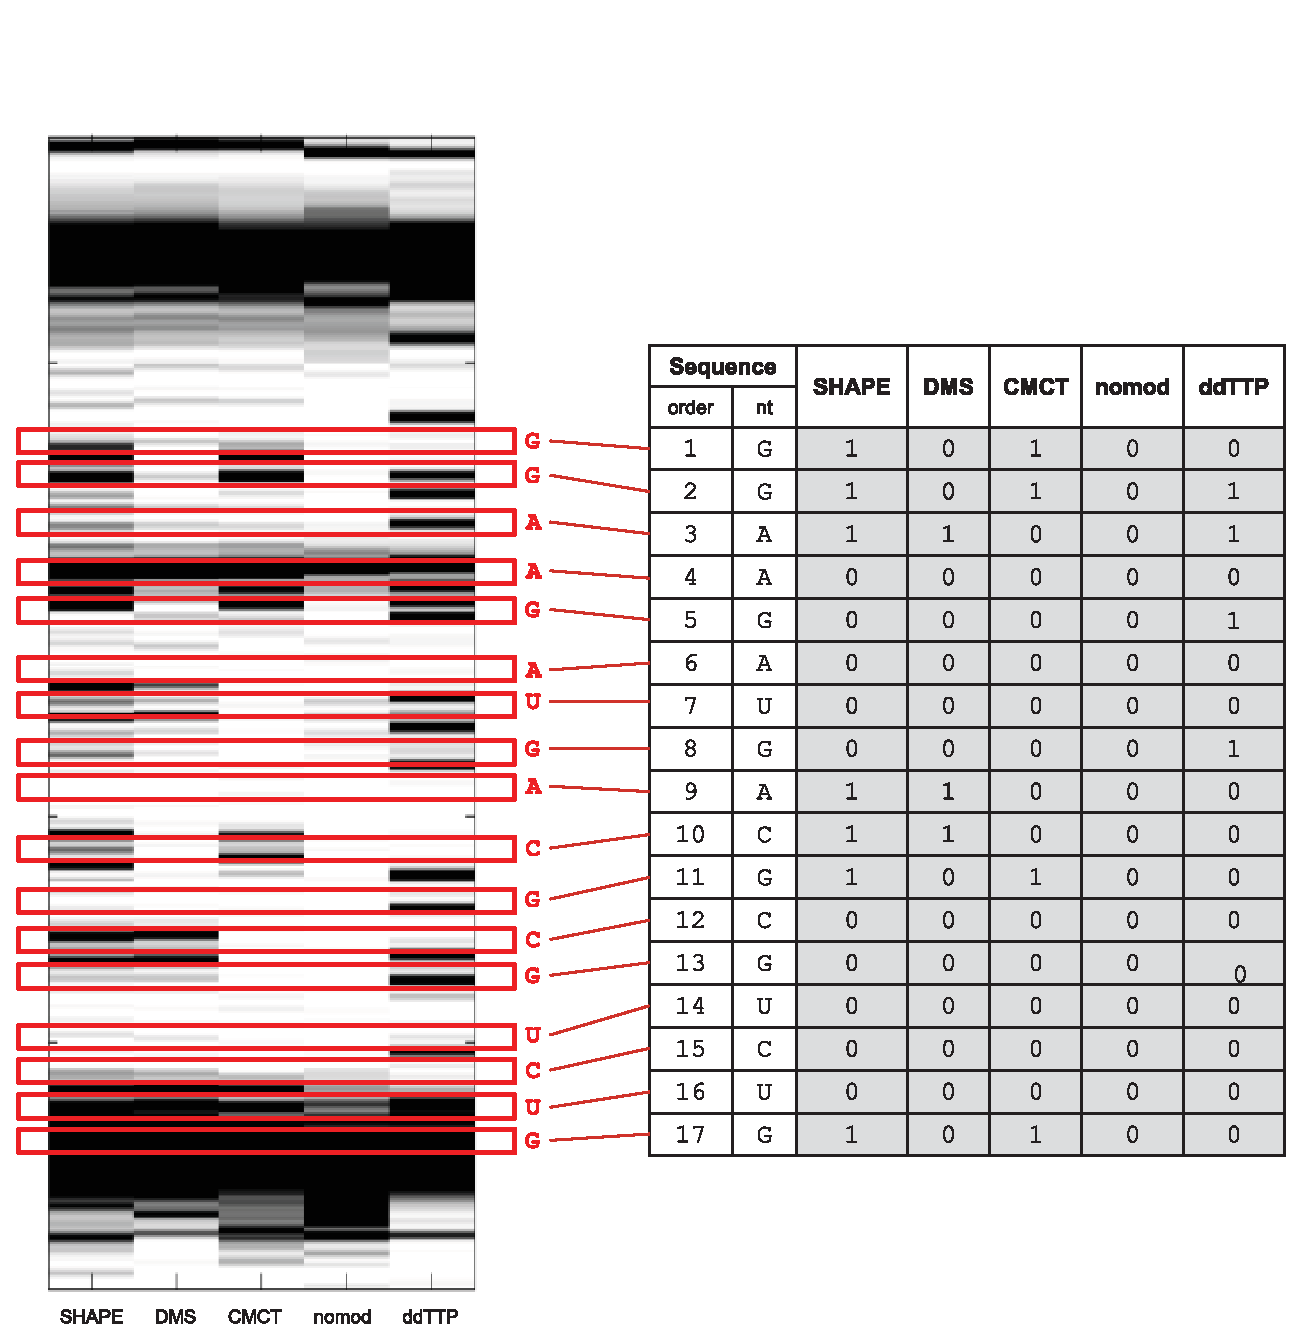
\includegraphics[width=\linewidth]{figures/supp_band_annotation_example}
\caption{\hilight{An example of band annotation. The left figure illustrates five profiles (SHAPE, DMS, CMCT, nomod, ddTTP) of CE data and an example of their band annotaion. Each band location is directed by red line from the corresponding row (nucleotide) of the prediction matrix on the right side. Basically the objective of band annotation is to determine band locations such that the ones in the prediction matrix correspond to high intensity values, and zeros to low values. It is also important to keep the locations fairly evenly distributed on the entire profile, as in this figure.} }
\label{f:old_vs_new}
\end{figure}
%%%%%%%%%%%%%%%%%%%%%%%%%%%%%%%%%%%%%%%%%%%%%%%%%%%%%%%%%%%%%%%%%%%%%%%%%%%%%%%%


%%%%%%%%%%%%%%%%%%%%%%%%%%%%%%%%%%%%%%%%%%%%%%%%%%%%%%%%%%%%%%%%%%%%%%%%%%%%%%%%
% OLD VS NEW
%%%%%%%%%%%%%%%%%%%%%%%%%%%%%%%%%%%%%%%%%%%%%%%%%%%%%%%%%%%%%%%%%%%%%%%%%%%%%%%%
\begin{figure}
\centering
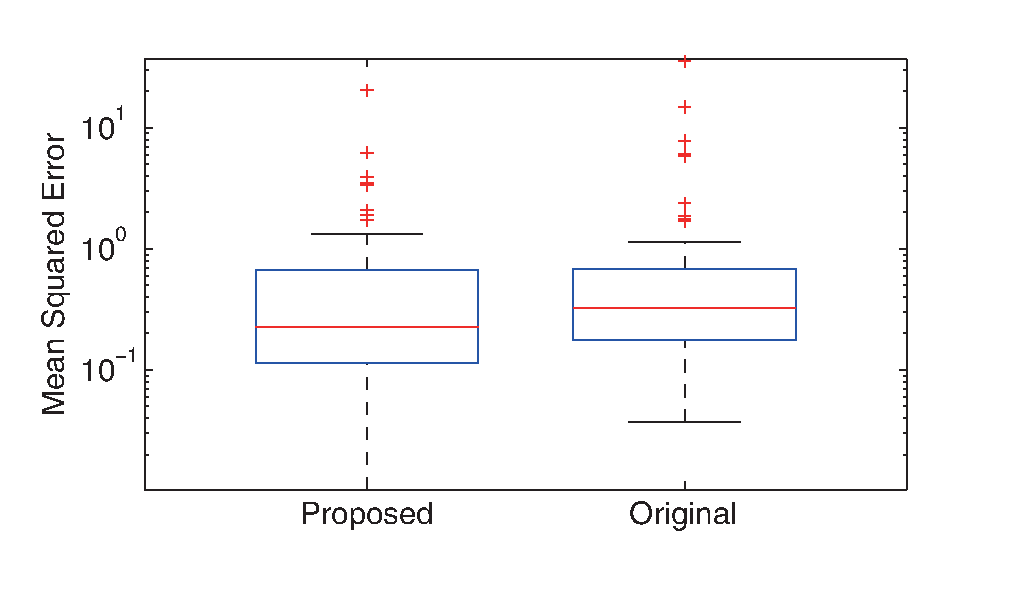
\includegraphics[width=\linewidth]{figures/supp_old_new_comparison}
\caption{The distribution of mean squared error (MSE) for the results from the proposed method and an older method without explicit peak-matching, respectively, over the 95 data sets. MSE units are normalized so that average distance between band locations is unity.}
\label{f:old_vs_new}
\end{figure}
%%%%%%%%%%%%%%%%%%%%%%%%%%%%%%%%%%%%%%%%%%%%%%%%%%%%%%%%%%%%%%%%%%%%%%%%%%%%%%%%


%%%%%%%%%%%%%%%%%%%%%%%%%%%%%%%%%%%%%%%%%%%%%%%%%%%%%%%%%%%%%%%%%%%%%%%%%%%%%%%%
% ETERNA COMPARISON
%%%%%%%%%%%%%%%%%%%%%%%%%%%%%%%%%%%%%%%%%%%%%%%%%%%%%%%%%%%%%%%%%%%%%%%%%%%%%%%%
\begin{figure}
\centering
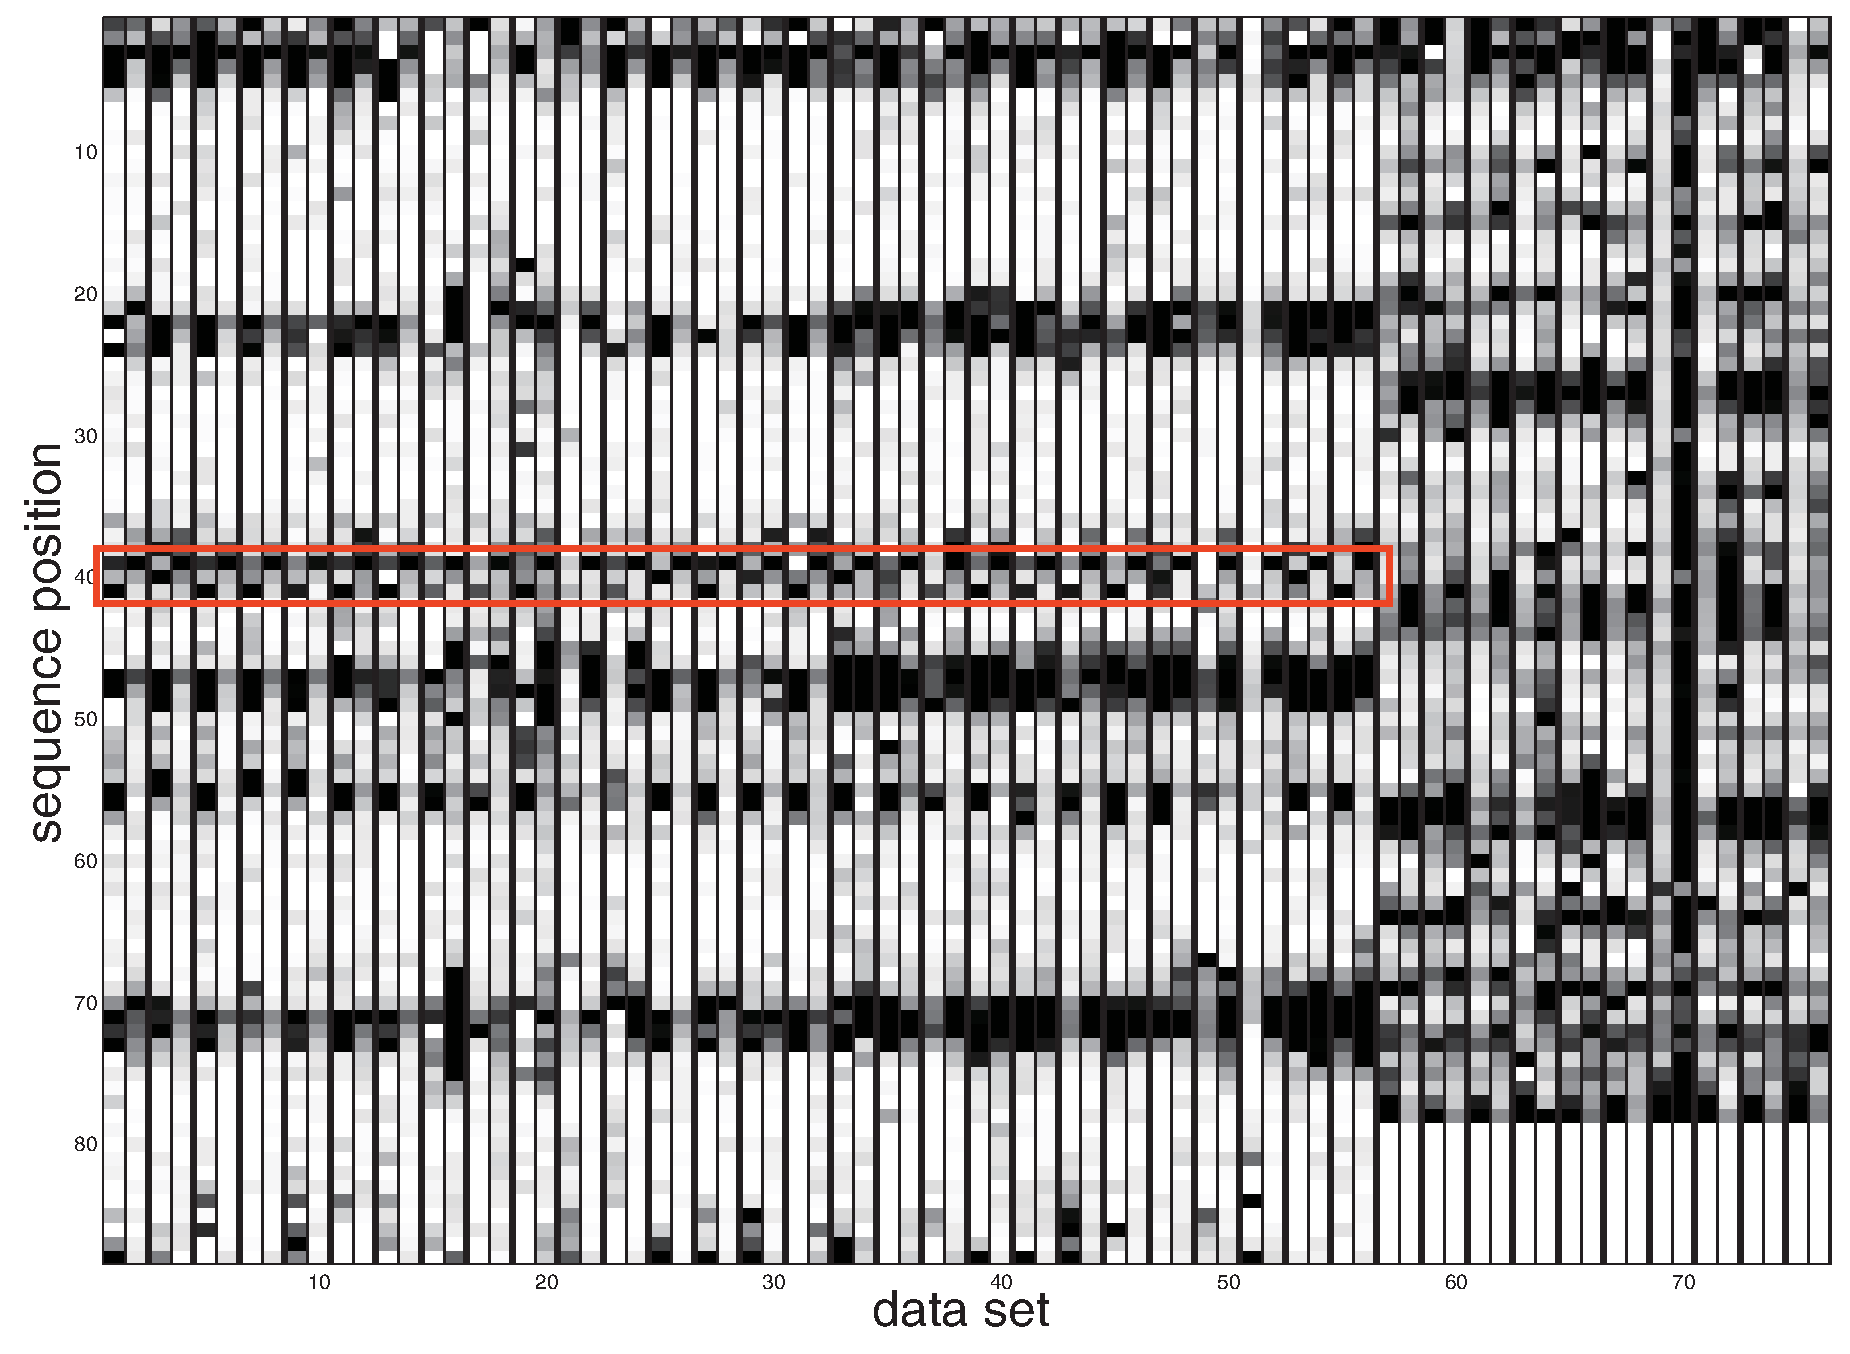
\includegraphics[width=\linewidth]{figures/supp_eterna_comparison}
\caption{Reactivity results from CE analysis and Illumina (next-generation-sequencing)-based structure mapping experiments, over 38 data sets from the EteRNA project. The heatmap presents results from two methods, presented in alternating order from left to right on each RNA sequence; CE analysis results are presented on odd numbered x-positions and Illlumina results are shown on even numbered x-positions. Visual inspection suggests concordance over most positions, except in the rectangular region. The original manually band-annotated CE data and Illumina data consistently show the highest intensity at different positions (41 and 39, respectively) higlighting an error in the manual CE annotation.}
\label{f:eterna_comparison}
\end{figure}


%%%%%%%%%%%%%%%%%%%%%%%%%%%%%%%%%%%%%%%%%%%%%%%%%%%%%%%%%%%%%%%%%%%%%%%%%%%%%%%%
% MULTIPLE VS SINGLE
%%%%%%%%%%%%%%%%%%%%%%%%%%%%%%%%%%%%%%%%%%%%%%%%%%%%%%%%%%%%%%%%%%%%%%%%%%%%%%%%
\begin{figure}
\centering
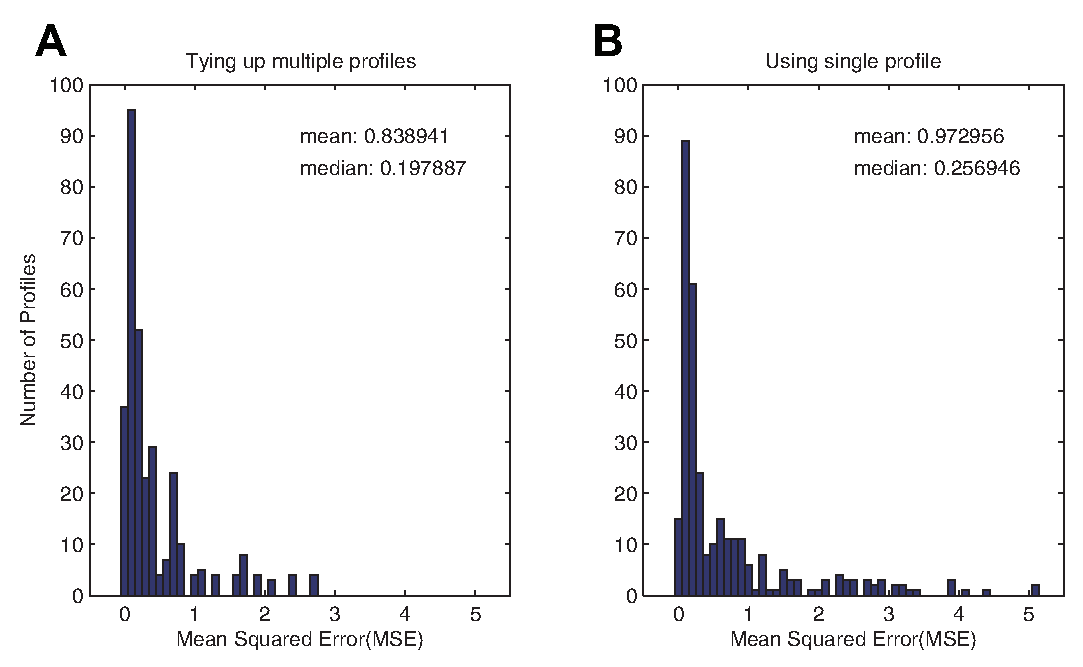
\includegraphics[width=\linewidth]{figures/supp_multiple_vs_single}
\caption{\hilight{The use of multiple profiles is one of the most important features of the proposed method. In order to quantitatively measure the benifit from taking more than one profiles as input, we visualized the distribution of MSEs on every profiles: the left histogram represents the distribution of MSEs when the proposed method takes multiple profiles as input at the same time, whereas the other represents the same distribution when only single profile is taken into account each time. Clearly, unacceptably high MSEs are less likely to be seen in the left histogram compared to the right one, supporting our claim that the use of multiple profiles enhances the quality of results of the proposed method.}}
\label{f:multiple_vs_single}
\end{figure}
%%%%%%%%%%%%%%%%%%%%%%%%%%%%%%%%%%%%%%%%%%%%%%%%%%%%%%%%%%%%%%%%%%%%%%%%%%%%%%%%


%%%%%%%%%%%%%%%%%%%%%%%%%%%%%%%%%%%%%%%%%%%%%%%%%%%%%%%%%%%%%%%%%%%%%%%%%%%%%%%
% HDV RESULT DETAIL
%%%%%%%%%%%%%%%%%%%%%%%%%%%%%%%%%%%%%%%%%%%%%%%%%%%%%%%%%%%%%%%%%%%%%%%%%%%%%%%
\begin{figure}
\centering
	\psfrag{r}[][][0.5]{$\rho$}
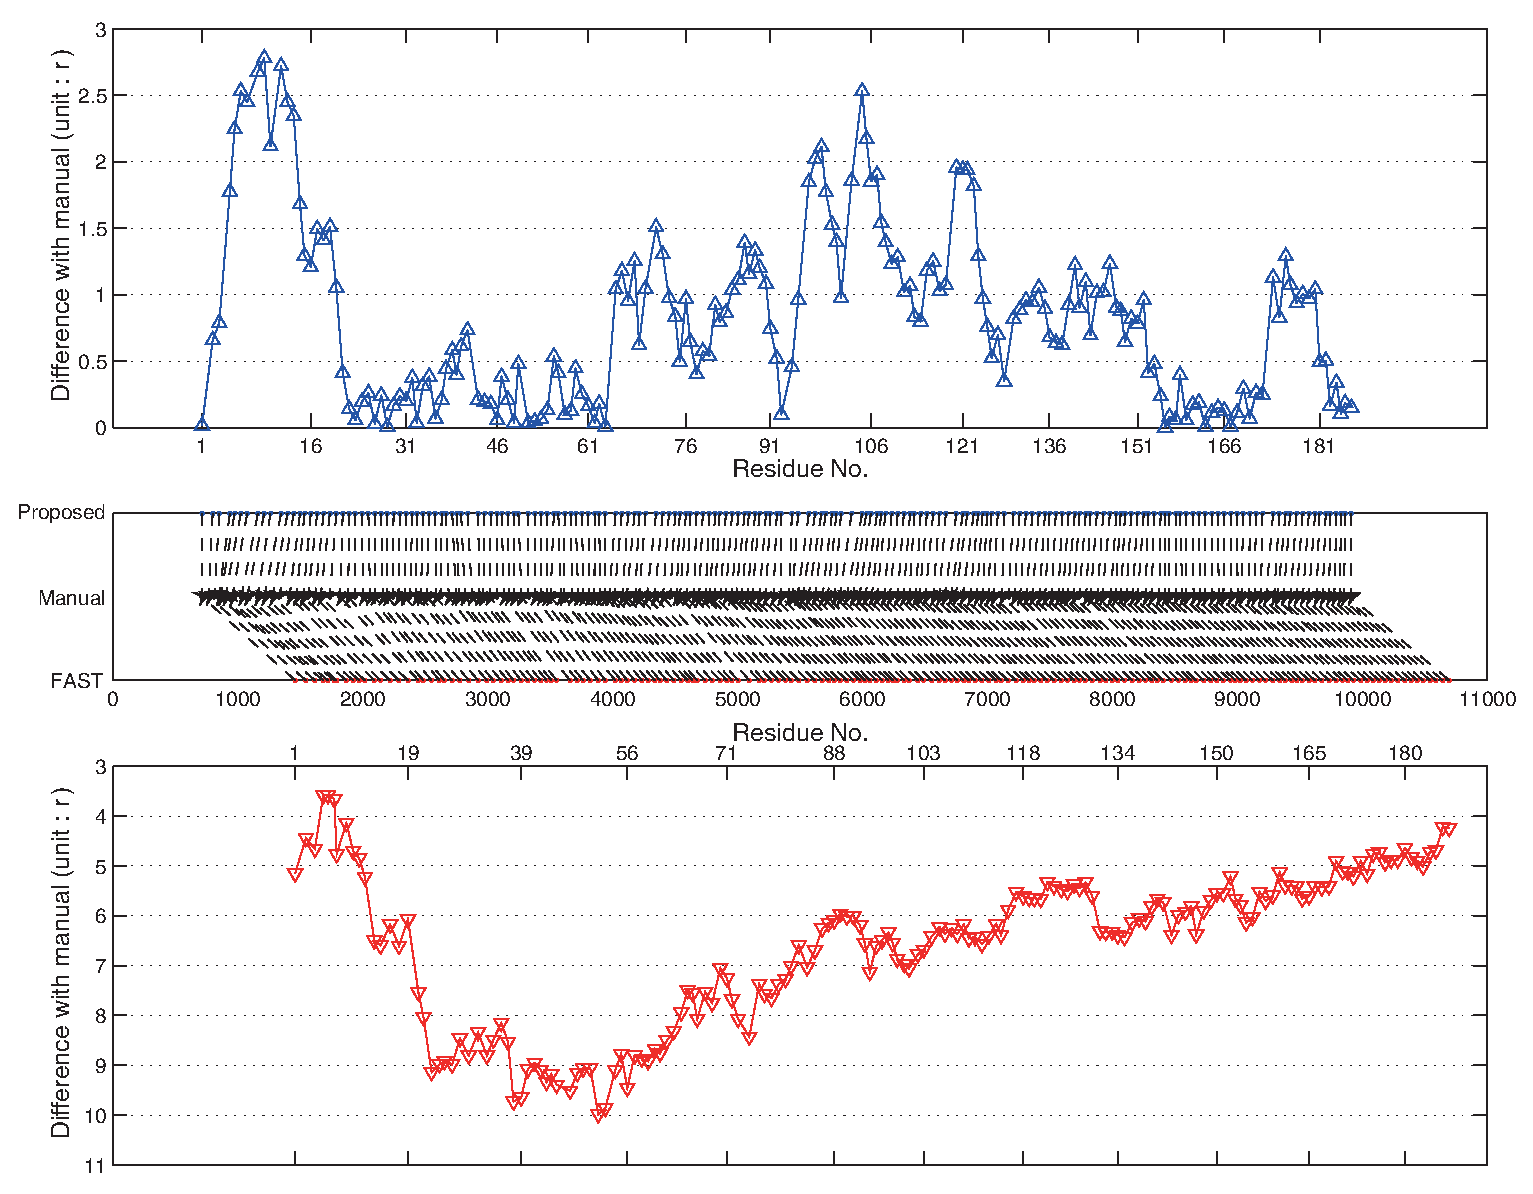
\includegraphics[width=\linewidth]{figures/result_hdv_result_detail2}
\caption{Error in band positions with respect to the reference band locations for 187-nt HDV data. Upper plot: error over residue positions for the proposed method; middle: mapping between the reference and computationally predicted band locations; lower: error over residue positions for FAST.}
\label{f:hdv-result-detail}
\end{figure}
%%%%%%%%%%%%%%%%%%%%%%%%%%%%%%%%%%%%%%%%%%%%%%%%%%%%%%%%%%%%%%%%%%%%%%%%%%%%%%%



\onecolumn

%%%%%%%%%%%%%%%%%%%%%%%%%%%%%%%%%%%%%%%%%%%%%%%%%%%%%%%%%%%%%%%%%%%%%%%%%%%%%%%
% TABLE: 95 DATA SETS RESULT
%%%%%%%%%%%%%%%%%%%%%%%%%%%%%%%%%%%%%%%%%%%%%%%%%%%%%%%%%%%%%%%%%%%%%%%%%%%%%%%

\begin{center}
\begin{longtable}{l ccc}

\caption{Name of data set and corresponding results respectively from the proposed method and QuShape, along with $\escore$-score.} \label{t:95_data_sets} \\
 & & \multicolumn{2}{c}{MSE} \\
Data Set Name & $\escore$-score & \multicolumn{1}{c}{proposed} & QuShape \\\hline
\endfirsthead

%\multicolumn{4}{l}{\textit{Continued from previous page}} \\
 & & \multicolumn{2}{c}{MSE} \\
Data Set Name & $\escore$-score & \multicolumn{1}{c}{proposed} & QuShape \\\hline
\endhead

\\
\multicolumn{4}{r}{\textit{Continued on next page}} \\
\endfoot
\endlastfoot


Fragments of Old Winners		&1.00	&0.80	&2.38 \\
FNM Apatamet 1st try			&1.00 	&0.55 	&0.86 \\
Freywa - Cross FMN - Reshiram	&1.00 	&0.22 	&0.68 \\
wisdave's apatamer \#1			&1.00 	&0.24 	&0.38 \\
Fiskers single aptamer 2		&0.97 	&1.13 	&1.49 \\
Starry's Single III			&1.00 	&0.10 	&1.78 \\
fold vs shapes				&1.00 	&0.18 	&0.15 \\
ViennaRNA design 01			&0.88 	&0.49 	&0.74 \\
ViennaRNA design 03			&1.00 	&0.12 	&1.11 \\
ViennaRNA design 04			&1.00 	&0.10 	&0.33 \\
NUPACK design 02				&0.53 	&4.73 	&66.49 \\
NUPACK design 04				&0.88 	&0.52 	&1.88 \\
Freywa - Cross FMN R2 - Zekrom	&0.96 	&1.10 	&1.10 \\
Tadpole 2.0					&1.00 	&0.09 	&0.46 \\
Kiwi							&1.00 	&0.18 	&0.51 \\
LROppy 93.4\% FMN				&1.00 	&0.07 	&1.26 \\
EteRNA ensemble design 01 (L2)	&0.85 	&2.38 	&4.95 \\
EteRNA ensemble design 02 (L2)	&1.00 	&0.18 	&7.60 \\
EteRNA ensemble design 03 (L2)	&0.99 	&0.18 	&0.74 \\
EteRNA ensemble design 04 (L2)	&0.97 	&0.39 	&0.34 \\
EteRNA ensemble design 05 (sparse 5)		&0.99 	&0.05 	&0.55 \\
EteRNA ensemble design 06 (sparse 5)		&0.94 	&0.40 	&1.70 \\
EteRNA ensemble design 07 (sparse 5)		&0.97 	&0.36 	&6.38 \\
EteRNA ensemble design 08 (sparse 5)		&1.00 	&0.10 	&0.18 \\
EteRNA ensemble design 09 (conventional)		&0.91 	&1.68 	&1.06 \\
EteRNA ensemble design 10 (conventional)		&0.82 	&0.58 	&1.48 \\
EteRNA ensemble design 11 (conventional)		&0.99 	&0.15 	&0.58 \\
EteRNA ensemble design 12 (conventional)		&1.00 	&0.13 	&0.36 \\
Brourd - FMNA 1			&1.00 	&0.08 	&0.40 \\
The Revolution of the Mobile Archer	&1.00 	&0.19 	&0.75 \\
Fragments of old Winners (3)	&0.94 	&1.05 	&5.13 \\
Smart Solution				&1.00 	&0.05 	&0.07 \\
Lump In My Throat				&0.94 	&0.85 	&7.12 \\
JP-14-0-17 (FMN-SBS II)		&0.94 	&0.34 	&0.30 \\
SBSII-2						&0.87 	&0.56 	&6.44 \\
Mod of Quasispecies design Fragments of old winners	&0.87 	&0.48 	&7.35 \\
NUPACK design 01				&0.74 	&21.50 	&62.22 \\
NUPACK design 02				&0.90 	&1.70 	&16.09 \\
NUPACK design 03				&0.90 	&0.89 	&46.15 \\
NUPACK design 04				&0.84 	&1.09 	&5.58 \\
ViennaRNA design 01			&0.81 	&2.18 	&0.51 \\
ViennaRNA design 02			&0.84 	&0.20 	&0.36 \\
ViennaRNA design 03			&0.84 	&0.05 	&0.84 \\
NUPACK design 01				&0.84 	&0.45 	&0.20 \\
NUPACK design 02				&0.87 	&1.36 	&3.30 \\
NUPACK design 03				&0.90 	&1.70 	&0.34 \\
NUPACK design 04				&0.90 	&9.63 	&0.72 \\
ViennaRNA design 01			&0.84 	&3.20 	&0.67 \\
ViennaRNA design 03			&0.81 	&0.06 	&0.25 \\
Fragments of Old Winners (4)	&1.00 	&0.09 	&0.21 \\
GOOD SOLUTION					&1.00 	&0.15 	&0.57 \\
Mod of Quasispecies design Fragments of old winners v2		&0.87 	&1.01 	&10.48 \\
Combo - improved				&1.00 	&0.12 	&0.30 \\
EteRNA ensemble design 0 (sparse 5) 		&1.00 	&0.08 	&0.59 \\
EteRNA ensemble design 1 (sparse 5)		&0.97 	&0.20 	&0.75 \\
EteRNA ensemble design 2 (sparse 5)		&1.00 	&0.18 	&0.75 \\
EteRNA ensemble design 3 (sparse 5)		&0.97 	&0.06 	&0.28 \\
EteRNA ensemble design 4 (L2)		&1.00 	&0.02 	&0.20 \\
EteRNA ensemble design 5 (L2)		&0.97 	&0.34 	&0.78 \\
EteRNA ensemble design 6 (L2)		&0.97 	&0.13 	&0.68 \\
EteRNA ensemble design 7 (L2)		&1.00 	&0.17 	&0.34 \\
EteRNA ensemble design 08 (conventional)		&1.00 	&0.05 	&0.21 \\
EteRNA ensemble design 09 (conventional)		&0.97 	&0.15 	&0.66 \\
EteRNA ensemble design 10 (conventional)		&1.00 	&0.61 	&0.65 \\
EteRNA ensemble design 11 (conventional)		&1.00 	&0.15 	&0.27 \\
Wild Cross - 	2				&0.94 	&0.12 	&0.72 \\
Mod of JerryP70				&1.00 	&0.07 	&0.55 \\
Mod of brourds 1 st round -		&0.84 	&0.08 	&0.88 \\
Unique Stacks					&0.93 	&0.24 	&0.54 \\
G-C pairs in multloops in same direction		&0.98 	&0.04 	&1.38 \\
Fisker's Binding branches		&0.93 	&0.12 	&0.76 \\
NUPACK design 01				&0.95 	&0.25 	&0.93 \\
NUPACK design 02				&0.93 	&0.53 	&0.39 \\
NUPACK design 03				&0.93 	&3.05 	&1.41 \\
NUPACK design 04				&0.98 	&0.43 	&0.39 \\
ViennaRNA design 04			&0.88 	&0.40 	&0.48 \\
EteRNA ensemble design 02 (conventional)		&0.95 	&1.80 	&1.35 \\
EteRNA ensemble design 04 (conventional)		&1.00 	&0.03 	&0.45 \\
EteRNA ensemble design 05 (sparse 5)		&1.00 	&0.06 	&0.05 \\
EteRNA ensemble design 06 (sparse 5)		&1.00 	&0.26 	&0.41 \\
EteRNA ensemble design 07 (sparse 5)		&0.98 	&0.19 	&0.39 \\
EteRNA ensemble design 08 (sparse 5)		&0.99 	&0.12 	&0.10 \\
EteRNA ensemble design 09 (L2)		&1.00 	&0.28 	&13.50 \\
EteRNA ensemble design 11 (L2)		&0.98 	&0.21 	&0.18 \\
EteRNA ensemble design 12 (L2)		&0.99 	&0.08 	&0.23 \\
UUU / GCA Triloops (Round 2)	&0.91 	&0.69 	&3.00 \\
Uracil in 1-2 x2				&0.85 	&0.12 	&0.79 \\
1 U-leg, 1 A-leg				&0.94 	&1.01 	&3.98 \\
Bonus Army					&0.91 	&0.23 	&0.86 \\
wisdave's 2nd round			&0.76 	&0.68 	&1.02 \\
C - BACK						&0.88 	&1.24 	&0.24 \\
Beauty in Balance				&0.97 	&0.13 	&1.33 \\
Very Low Entropy <0.6 T-B-C \#5	&0.94 	&0.09 	&0.16 \\
Improves on Quasispecies UUU/GCA Triloop	&0.91 	&0.08 	&0.06 \\
sta1							&0.82 	&0.21 	&1.86 \\

\end{longtable}
\end{center}



\newpage



%%%%%%%%%%%%%%%%%%%%%%%%%%%%%%%%%%%%%%%%%%%%%%%%%%%%%%%%%%%%%%%%%%%%%%%%%%%%%%%
% TABLE: ADDITIONAL, LONGER DATA RESULT
%%%%%%%%%%%%%%%%%%%%%%%%%%%%%%%%%%%%%%%%%%%%%%%%%%%%%%%%%%%%%%%%%%%%%%%%%%%%%%%

\begin{center}
\begin{longtable}{l cccc}

\caption{Description of longer data sets and results from the tests with these data sets. $^a$An extraordinary result mainly caused by a misalignment between profiles.} \label{t:additional_data_sets} \\

Name & \# profiles & \# bands per profile & MSE & $\escore$-score \\
\hline
\endfirsthead
Name & \# profiles & \# bands per profile & MSE & $\escore$-score \\
\endhead
\endfoot
%{$^a$An extraordinary result mainly caused by a misalignment between profiles (to be discussed in the discussion section) }
\endlastfoot

GIR1 noref 	& 21 & 199 & 0.09 & 0.99 \\
GIR1 ref 		& 21 & 225 & 0.12 & 0.98 \\
AdoCbl noref 	& 16 & 179 & 0.61 & 0.97 \\
AdoCbl ref 	& 16 & 205 & 0.68 & 0.90 \\
VS noref 		& 48 & 195 & 0.16 & 0.96 \\
VS ref 		& 48 & 233 & 0.12 & 0.96 \\
SAM noref 	& 32 & 103 & 0.09 & 0.96 \\
SAM ref 		& 32 & 143 & 0.09 & 0.96 \\
HTP noref 	& 32 & 79  & 0.05 & 1.00 \\
HTP ref 		& 32 & 116 & 0.05 & 1.00 \\
Tbox 		& 20 & 141 & 0.34 & 0.98 \\
tRNA 		& 20 & 119 & 0.63 & 0.83 \\
cdiAMP 		& 36 & 171 & 0.16 & 0.99 \\
16S 			& 8  & 125 & 0.21 & 0.98 \\
C19 			& 16 & 319 & 0.18 & 0.99 \\
tC19 		& 16 & 248 & 0.01 & 1.00 \\
tC19Z 		& 16 & 248 & 0.01 & 0.99 \\
C1Lig 		& 7  & 167 & 0.04 & 1.00 \\
Hox5 		& 9  & 261 & 0.11 & 0.99 \\
Hox9D 		& 16 & 296 & 0.44 & 0.99 \\
L-21			& 20 & 413 & 2.00$^a$ & 0.98 \\
\end{longtable}
\end{center}



\newpage


%%%%%%%%%%%%%%%%%%%%%%%%%%%%%%%%%%%%%%%%%%%%%%%%%%%%%%%%%%%%%%%%%%%%%%%%%%%%%%%
% TABLE: PEAK DECONVOLUTION
%%%%%%%%%%%%%%%%%%%%%%%%%%%%%%%%%%%%%%%%%%%%%%%%%%%%%%%%%%%%%%%%%%%%%%%%%%%%%%%

\begin{center}
\begin{longtable}{l ccc}

\caption{Name of data set and corresponding results respectively from the proposed method and manual annotation, along with the ratio between two MSE values (proposed / manual)} \label{t:peak_deconvolution} \\
 & & \multicolumn{2}{c}{MSE} \\
Data Set Name & ratio & \multicolumn{1}{c}{proposed} & manual \\\hline
\endfirsthead

%\multicolumn{4}{l}{\textit{Continued from previous page}} \\
 & & \multicolumn{2}{c}{MSE} \\
Data Set Name & ratio & \multicolumn{1}{c}{proposed} & manual \\\hline
\endhead

\\
\multicolumn{4}{r}{\textit{Continued on next page}} \\
\endfoot
\endlastfoot


Fragments of Old Winners		&1.15	&0.82	&0.71 \\
FNM Apatamet 1st try			&0.94 	&0.57 	&0.61 \\
Freywa - Cross FMN - Reshiram	&2.60 	&0.24 	&0.09 \\
wisdave's apatamer \#1			&1.32 	&0.26 	&0.20 \\
Fiskers single aptamer 2		&9.31 	&1.43 	&0.15 \\
Starry's Single III			&0.73 	&0.11 	&0.15 \\
fold vs shapes				&1.22 	&0.18 	&0.15 \\
ViennaRNA design 01			&0.97 	&0.58 	&0.60 \\
ViennaRNA design 03			&0.67 	&0.15 	&0.22 \\
ViennaRNA design 04			&1.04 	&0.09 	&0.09 \\
NUPACK design 02				&3.80 	&4.60 	&1.21 \\
NUPACK design 04				&10.10 	&3.18 	&0.32 \\
Freywa - Cross FMN R2 - Zekrom	&3.31	&0.98 	&0.30 \\
Tadpole 2.0					&1.77 	&0.10 	&0.06 \\
Kiwi							&4.07 	&0.11 	&0.03 \\
LROppy 93.4\% FMN				&2.07 	&0.09 	&0.04 \\
EteRNA ensemble design 01 (L2)	&5.33 	&4.27 	&0.80 \\
EteRNA ensemble design 02 (L2)	&3.03 	&0.19 	&0.06 \\
EteRNA ensemble design 03 (L2)	&1.12 	&0.22 	&0.19 \\
EteRNA ensemble design 04 (L2)	&1.47 	&0.39 	&0.26 \\
EteRNA ensemble design 05 (sparse 5)		&2.51 	&0.17 	&0.07 \\
EteRNA ensemble design 06 (sparse 5)		&1.91 	&0.58 	&0.31 \\
EteRNA ensemble design 07 (sparse 5)		&0.83 	&0.37 	&0.44 \\
EteRNA ensemble design 08 (sparse 5)		&5.90 	&0.75 	&0.13 \\
EteRNA ensemble design 09 (conventional)		&13.01 	&1.69 	&0.13 \\
EteRNA ensemble design 10 (conventional)		&1.16 	&1.01 	&0.87 \\
EteRNA ensemble design 11 (conventional)		&1.86 	&0.17 	&0.09 \\
EteRNA ensemble design 12 (conventional)		&2.51 	&0.23 	&0.09 \\
UUU / GCA Triloops (Round 2)	&40.59 	&0.51 	&0.01 \\
Uracil in 1-2 x2				&1.20 	&0.12 	&0.10 \\
1 U-leg, 1 A-leg				&3.62 	&1.19 	&0.33 \\
Bonus Army					&1.61 	&0.39 	&0.21 \\
wisdave's 2nd round			&12.73 	&0.74 	&0.06 \\
C - BACK						&2.75	&1.19 	&0.43 \\
Beauty in Balance				&9.22 	&1.36 	&0.15 \\
Very Low Entropy <0.6 T-B-C \#5	&1.36 	&0.14 	&0.11 \\
Improves on Quasispecies UUU/GCA Triloop	&11.22 	&0.08 	&0.01 \\
sta1							&1.09 	&0.23 	&0.21 \\

\end{longtable}
\end{center}





\newpage


%%%%%%%%%%%%%%%%%%%%%%%%%%%%%%%%%%%%%%%%%%%%%%%%%%%%%%%%%%%%%%%%%%%%%%%%%%%%%%%
% TABLE 3
%%%%%%%%%%%%%%%%%%%%%%%%%%%%%%%%%%%%%%%%%%%%%%%%%%%%%%%%%%%%%%%%%%%%%%%%%%%%%%%

\begin{center}
\begin{longtable}{lccc}

\caption{Name and type of data profile, and the Pearson's correlation coefficients between manually quantified areas, and those quantified by the proposed method and by QuShape respectively. Average values are posted for the multiple results from repetitive experiments with same data.} \\
 & & \multicolumn{2}{c}{correlation (averaged)} \\
Data Set Name & Data Type & proposed & QuShape \\\hline
\endfirsthead

%\multicolumn{4}{l}{\textit{Continued from previous page}} \\
 & & \multicolumn{2}{c}{correlation (averaged)} \\
Data Set Name & Data Type & proposed & QuShape \\\hline
\endhead

\\
\multicolumn{4}{r}{\textit{Continued on next page}} \\
\endfoot
\endlastfoot

Fragments of Old Winners	&	DMS	&	0.9383 	&	0.9654 	\\
FNM Apatamet 1st try	&	DMS	&	0.6913 	&	0.9468 	\\
Freywa - Cross FMN - Reshiram	&	DMS	&	0.9750 	&	0.9433 	\\
wisdave's apatamer \#1	&	DMS	&	0.9796 	&	0.9546 	\\
Fiskers single aptamer 2	&	DMS	&	0.9708 	&	0.9588 	\\
Starry''s Single III	&	DMS	&	0.9788 	&	0.7297 	\\
fold vs shapes	&	DMS	&	0.9890 	&	0.9880 	\\
ViennaRNA design 01	&	DMS	&	0.9927 	&	0.9745 	\\
ViennaRNA design 03	&	DMS	&	0.9957 	&	0.9929 	\\
ViennaRNA design 04	&	DMS	&	0.9667 	&	0.9232 	\\
NUPACK design 02	&	DMS	&	0.9148 	&	0.8848 	\\
NUPACK design 04	&	DMS	&	0.9557 	&	0.7359 	\\
Freywa - Cross FMN R2 - Zekrom	&	DMS	&	0.9832 	&	0.7436 	\\
Tadpole 2.0	&	DMS	&	0.9757 	&	0.9444 	\\
Kiwi	&	DMS	&	0.9964 	&	0.8889 	\\
LROppy 93.4\% FMN	&	DMS	&	0.9899 	&	0.9422 	\\
EteRNA ensemble design 01 (L2)	&	DMS	&	0.9935 	&	0.9917 	\\
EteRNA ensemble design 02 (L2)	&	DMS	&	0.9650 	&	0.8977 	\\
EteRNA ensemble design 03 (L2)	&	DMS	&	0.9215 	&	0.9130 	\\
EteRNA ensemble design 04 (L2)	&	DMS	&	0.9145 	&	0.9482 	\\
EteRNA ensemble design 05 (Sparse 5)	&	DMS	&	0.9835 	&	0.9616 	\\
EteRNA ensemble design 06 (Sparse 5)	&	DMS	&	0.9889 	&	0.9822 	\\
EteRNA ensemble design 07 (sparse 5)	&	DMS	&	0.9452 	&	0.8044 	\\
EteRNA ensemble design 08 (sparse 5)	&	DMS	&	0.9752 	&	0.9748 	\\
EteRNA ensemble design 09 (conventional)	&	DMS	&	0.5389 	&	0.6876 	\\
EteRNA ensemble design 10 (conventional)	&	DMS	&	0.9898 	&	0.9867 	\\
EteRNA ensemble design 11 (conventional)	&	DMS	&	0.9962 	&	0.9480 	\\
EteRNA ensemble design 12 (conventional)	&	DMS	&	0.9882 	&	0.9109 	\\
Brourd - FMNA 1	&	SHAPE	&	0.9747 	&	0.9480 	\\
Brourd - FMNA 1	&	DMS	&	0.9908 	&	0.7227 	\\
The Revolution of the Mobile Archer	&	SHAPE	&	0.9897 	&	0.9360 	\\
The Revolution of the Mobile Archer	&	DMS	&	0.9816 	&	0.9785 	\\
Fragments of old Winners (3)	&	SHAPE	&	0.9942 	&	0.9756 	\\
Fragments of old Winners (3)	&	DMS	&	0.9976 	&	0.9868 	\\
Smart Solution	&	SHAPE	&	0.9903 	&	0.9883 	\\
Smart Solution	&	DMS	&	0.9942 	&	0.8834 	\\
Lump In My Throat	&	SHAPE	&	0.9529 	&	0.9545 	\\
Lump In My Throat	&	DMS	&	0.9904 	&	0.7225 	\\
JP-14-0-17 (FMN-SBS II)	&	SHAPE	&	0.9441 	&	0.9762 	\\
JP-14-0-17 (FMN-SBS II)	&	DMS	&	0.9827 	&	0.9684 	\\
SBSII-2	&	SHAPE	&	0.9177 	&	0.9057 	\\
SBSII-2	&	DMS	&	0.9570 	&	0.9093 	\\
Mod of Quasispecies design Fragments of old winners	&	SHAPE	&	0.9422 	&	0.9724 	\\
Mod of Quasispecies design Fragments of old winners	&	DMS	&	0.9649 	&	0.4340 	\\
NUPACK design 01	&	SHAPE	&	0.9675 	&	0.9706 	\\
NUPACK design 01	&	DMS	&	0.9858 	&	0.9842 	\\
NUPACK design 02	&	SHAPE	&	0.8283 	&	0.5124 	\\
NUPACK design 02	&	DMS	&	0.9225 	&	0.4406 	\\
NUPACK design 03	&	SHAPE	&	0.9465 	&	0.9102 	\\
NUPACK design 03	&	DMS	&	0.9987 	&	0.9978 	\\
NUPACK design 04	&	SHAPE	&	0.9990 	&	0.9898 	\\
NUPACK design 04	&	DMS	&	0.9995 	&	0.9657 	\\
ViennaRNA design 01	&	SHAPE	&	0.7068 	&	0.7119 	\\
ViennaRNA design 01	&	DMS	&	0.9524 	&	0.5016 	\\
ViennaRNA design 02	&	SHAPE	&	0.8846 	&	0.7067 	\\
ViennaRNA design 02	&	DMS	&	0.9773 	&	0.6991 	\\
ViennaRNA design 03	&	SHAPE	&	0.9866 	&	0.7357 	\\
ViennaRNA design 03	&	DMS	&	0.9806 	&	0.7832 	\\
NUPACK design 01	&	SHAPE	&	0.8479 	&	0.8934 	\\
NUPACK design 01	&	DMS	&	0.9871 	&	0.9948 	\\
NUPACK design 02	&	SHAPE	&	0.8883 	&	0.7229 	\\
NUPACK design 02	&	DMS	&	0.9475 	&	0.9425 	\\
NUPACK design 03	&	SHAPE	&	0.6236 	&	0.8557 	\\
NUPACK design 03	&	DMS	&	0.9437 	&	0.9545 	\\
NUPACK design 04	&	SHAPE	&	0.8638 	&	0.7790 	\\
NUPACK design 04	&	DMS	&	0.9835 	&	0.8958 	\\
ViennaRNA design 01	&	SHAPE	&	0.9422 	&	0.7428 	\\
ViennaRNA design 01	&	DMS	&	0.9710 	&	0.9098 	\\
ViennaRNA design 03	&	SHAPE	&	0.9845 	&	0.9231 	\\
ViennaRNA design 03	&	DMS	&	0.9950 	&	0.9144 	\\
Fragments of Old Winners (4)	&	SHAPE	&	0.9743 	&	0.9742 	\\
Fragments of Old Winners (4)	&	DMS	&	0.9932 	&	0.9890 	\\
GOOD SOLUTION	&	SHAPE	&	0.9518 	&	0.9355 	\\
GOOD SOLUTION	&	DMS	&	0.9840 	&	0.9714 	\\
Mod of Quasispecies design Fragments of old winners v2	&	SHAPE	&	0.5981 	&	0.6670 	\\
Mod of Quasispecies design Fragments of old winners v2	&	DMS	&	0.5231 	&	0.9051 	\\
Combo - improved	&	SHAPE	&	0.9483 	&	0.9111 	\\
Combo - improved	&	DMS	&	0.9960 	&	0.9854 	\\
EteRNA ensemble design 0 (sparse 5)	&	SHAPE	&	0.9528 	&	0.9265 	\\
EteRNA ensemble design 0 (sparse 5)	&	DMS	&	0.9814 	&	0.8917 	\\
EteRNA ensemble design 1 (sparse 5)	&	SHAPE	&	0.9179 	&	0.9152 	\\
EteRNA ensemble design 1 (sparse 5)	&	DMS	&	0.9547 	&	0.9228 	\\
EteRNA ensemble design 2 (sparse 5)	&	SHAPE	&	0.9322 	&	0.9145 	\\
EteRNA ensemble design 2 (sparse 5)	&	DMS	&	0.9506 	&	0.9029 	\\
EteRNA ensemble design 3 (sparse 5)	&	SHAPE	&	0.9961 	&	0.9217 	\\
EteRNA ensemble design 3 (sparse 5)	&	DMS	&	0.9965 	&	0.9216 	\\
EteRNA ensemble design 4 (L2)	&	SHAPE	&	0.9967 	&	0.9172 	\\
EteRNA ensemble design 4 (L2)	&	DMS	&	0.9895 	&	0.9782 	\\
EteRNA ensemble design 5 (L2)	&	SHAPE	&	0.6165 	&	0.4973 	\\
EteRNA ensemble design 5 (L2)	&	DMS	&	0.8898 	&	0.8574 	\\
EteRNA ensemble design 6 (L2)	&	SHAPE	&	0.9795 	&	0.9049 	\\
EteRNA ensemble design 6 (L2)	&	DMS	&	0.9885 	&	0.8338 	\\
EteRNA ensemble design 7 (L2)	&	SHAPE	&	0.9676 	&	0.9730 	\\
EteRNA ensemble design 7 (L2)	&	DMS	&	0.9512 	&	0.9526 	\\
EteRNA ensemble design 08 (conventional)	&	SHAPE	&	0.9904 	&	0.9249 	\\
EteRNA ensemble design 08 (conventional)	&	DMS	&	0.9947 	&	0.9326 	\\
EteRNA ensemble design 09 (conventional)	&	SHAPE	&	0.9413 	&	0.9193 	\\
EteRNA ensemble design 09 (conventional)	&	DMS	&	0.9930 	&	0.9218 	\\
EteRNA ensemble design 10 (conventional)	&	SHAPE	&	0.6075 	&	0.8549 	\\
EteRNA ensemble design 10 (conventional)	&	DMS	&	0.9651 	&	0.9046 	\\
EteRNA ensemble design 11 (conventional)	&	SHAPE	&	0.9865 	&	0.9857 	\\
EteRNA ensemble design 11 (conventional)	&	DMS	&	0.9881 	&	0.9845 	\\
Wild Cross - 2	&	SHAPE	&	0.9936 	&	0.7966 	\\
Wild Cross - 2	&	DMS	&	0.9957 	&	0.9414 	\\
Mod of JerryP70	&	SHAPE	&	0.9583 	&	0.9068 	\\
Mod of JerryP70	&	DMS	&	0.9960 	&	0.7095 	\\
Mod of brourds 1 st round -	&	SHAPE	&	0.9992 	&	0.8678 	\\
Mod of brourds 1 st round -	&	DMS	&	0.9998 	&	0.9901 	\\
Unique Stacks	&	SHAPE	&	0.9687 	&	0.8632 	\\
Unique Stacks	&	DMS	&	0.9832 	&	0.8142 	\\
G-C pairs in multloops in same direction	&	SHAPE	&	0.9857 	&	0.9698 	\\
G-C pairs in multloops in same direction	&	DMS	&	0.9972 	&	0.9866 	\\
Fisker's Binding branches	&	SHAPE	&	0.3513 	&	0.9764 	\\
Fisker's Binding branches	&	DMS	&	0.2634 	&	0.9424 	\\
NUPACK design 01	&	SHAPE	&	0.9909 	&	0.9591 	\\
NUPACK design 01	&	DMS	&	0.9958 	&	0.9836 	\\
NUPACK design 02	&	SHAPE	&	0.8850 	&	0.8366 	\\
NUPACK design 02	&	DMS	&	0.9646 	&	0.8545 	\\
NUPACK design 03	&	SHAPE	&	0.6981 	&	0.7560 	\\
NUPACK design 03	&	DMS	&	0.9497 	&	0.7813 	\\
NUPACK design 04	&	SHAPE	&	0.7580 	&	0.9667 	\\
NUPACK design 04	&	DMS	&	0.9234 	&	0.9888 	\\
ViennaRNA design 04	&	SHAPE	&	0.8825 	&	0.8842 	\\
ViennaRNA design 04	&	DMS	&	0.9937 	&	0.9872 	\\
EteRNA ensemble design 02 (conventional)	&	SHAPE	&	0.9477 	&	0.9561 	\\
EteRNA ensemble design 02 (conventional)	&	DMS	&	0.8835 	&	0.8607 	\\
EteRNA ensemble design 04 (conventional)	&	SHAPE	&	0.9796 	&	0.9433 	\\
EteRNA ensemble design 04 (conventional)	&	DMS	&	0.9903 	&	0.7494 	\\
EteRNA ensemble design 05 (sparse 5)	&	SHAPE	&	0.8986 	&	0.9915 	\\
EteRNA ensemble design 05 (sparse 5)	&	DMS	&	0.9937 	&	0.9961 	\\
EteRNA ensemble design 06 (sparse 5)	&	SHAPE	&	0.9553 	&	0.5474 	\\
EteRNA ensemble design 06 (sparse 5)	&	DMS	&	0.9612 	&	0.9208 	\\
EteRNA ensemble design 07 (sparse 5)	&	SHAPE	&	0.9885 	&	0.9736 	\\
EteRNA ensemble design 07 (sparse 5)	&	DMS	&	0.9533 	&	0.9637 	\\
EteRNA ensemble design 08 (sparse 5)	&	SHAPE	&	0.9738 	&	0.9753 	\\
EteRNA ensemble design 08 (sparse 5)	&	DMS	&	0.9775 	&	0.9060 	\\
EteRNA ensemble design 09 (L2)	&	SHAPE	&	0.9765 	&	0.9359 	\\
EteRNA ensemble design 09 (L2)	&	DMS	&	0.9843 	&	0.5745 	\\
EteRNA ensemble design 11 (L2)	&	SHAPE	&	0.8987 	&	0.9365 	\\
EteRNA ensemble design 11 (L2)	&	DMS	&	0.9417 	&	0.8063 	\\
EteRNA ensemble design 12 (L2)	&	SHAPE	&	0.9790 	&	0.9616 	\\
EteRNA ensemble design 12 (L2)	&	DMS	&	0.9649 	&	0.9511 	\\
UUU / GCA Triloops (Round 2)	&	SHAPE	&	0.9889 	&	0.8104 	\\
Uracil in 1-2 x2	&	SHAPE	&	0.9749 	&	0.9665 	\\
1 U-leg, 1 A-leg	&	SHAPE	&	0.8023 	&	0.6919 	\\
Bonus Army	&	SHAPE	&	0.9743 	&	0.7612 	\\
wisdave's 2nd round	&	SHAPE	&	0.9796 	&	0.8770 	\\
C - BACK	&	SHAPE	&	0.9705 	&	0.9441 	\\
Beauty in Balance	&	SHAPE	&	0.9879 	&	0.7477 	\\
Very Low Entropy <0.6 T-B-C \#5	&	SHAPE	&	0.9745 	&	0.8384 	\\
Improves on Quasispecies UUU/GCA Triloop	&	SHAPE	&	0.9849 	&	0.9971 	\\
sta1	&	SHAPE	&	0.9954 	&	0.9117 	\\

\end{longtable}
\end{center}







\twocolumn









%\bibliographystyle{natbib}
%\bibliographystyle{reference}
%\bibliographystyle{unsrt}
%\bibliography{reference}


\end{document}


